\documentclass[12pt,a4paper]{article}
\usepackage[utf8]{inputenc}
\usepackage{amsmath}
\usepackage{amsfonts}
\usepackage{amssymb}
\usepackage{graphicx}
\usepackage{xcolor}
\usepackage[top=1.5in,bottom=1in, left=1in, right=1in]{geometry}
\usepackage{fancyhdr}
\pagestyle{fancy}
\fancyhf{}
\rhead{\thepage}
\renewcommand{\headrulewidth}{0pt}
\usepackage{setspace}
\usepackage{hyperref}
\hypersetup{
  colorlinks   = true,
  urlcolor     = blue,
  linkcolor    = blue,
}
\usepackage{float}
\fancypagestyle{specialfooter}{%
  \fancyhf{}
  \renewcommand\headrulewidth{0pt}
  \fancyfoot[R]{CC-BY 4.0}
}

\usepackage{helvet}
\renewcommand{\familydefault}{\sfdefault}
\setlength{\parindent}{0em}
\setlength{\parskip}{1em}

\begin{document}
%\thispagestyle{empty}
\thispagestyle{specialfooter}
\onehalfspace

\begin{center}{\Large{\bfseries
Decentralized Privacy-Preserving\\
Proximity Tracing}\\[0.5cm]
Overview of Data Protection and Security}\\
Version: 3rd April 2020. Contact the first author for the latest version.\\[1cm]


\section*{Disclaimer/Provenance}

This document is a manually created, LaTeX version, of the original document at \url{https://github.com/DP-3T/documents/blob/master/DDP3T\%20-\%20Data\%20Protection\%20and\%20Security.pdf} as 
as captured on 2020-04-08. As this document was only available as a PDF it was hard to collaborate in typical Open Source style.

This\emph{ non-authoritative, derived}, version is to facilitate easier edits/contributions and collaboration.

See \url{https://github.com/DP-3T/} for the correct versions.
\end{center}

\pagebreak
\begin{center}{\Large{\bfseries
Decentralized Privacy-Preserving\\
Proximity Tracing}\\[0.5cm]
Overview of Data Protection and Security}\\
Version: 3rd April 2020. Contact the first author for the latest version.\\[1cm]


\textbf{EPFL} : Prof. Carmela Troncoso, Prof. Mathias Payer, Prof. Jean-Pierre\\
Hubaux, Prof. Marcel Salathé, Prof. James Larus, Prof. Edouard
Bugnion, Dr. Wouter Lueks, Theresa Stadler, Dr. Apostolos Pyrgelis, Dr.
Daniele Antonioli, Ludovic Barman, Sylvain Chatel


\textbf{ETHZ} : Prof. Kenneth Paterson, Prof. Srdjan Capkun, Prof. David Basin,
Dennis Jackson


\textbf{KU Leuven} : Prof. Bart Preneel, Prof. Nigel Smart, Dr. Dave Singelee,
Dr. Aysajan Abidin


\textbf{TU Delft} : Prof. Seda Guerses


\textbf{University College London} : Dr. Michael Veale


\textbf{CISPA} : Prof. Cas Cremers


\textbf{University of Oxford} : Dr. Reuben Binns


\textbf{TU Berlin / Fraunhofer HHI} : Prof. Thomas Wiegand
\end{center}
\clearpage
\singlespace \noindent
There is growing political and epidemiological interest in deploying technological approaches to help individuals and countries navigate the COVID-19 pandemic. One approach has been to make use of low-powered Bluetooth sensors on smartphones to inform users when they have been in contact with individuals who have since tested positive, and to support
epidemiologists with modelling efforts. However, some infrastructures that can enable
proportionate proximity tracing may fail to protect data, or be misused or extended far
beyond their initial purpose and beyond the lifetime of the crisis. This is all the more
important given the truly global nature of this challenge and the fact that the pandemic
crosses across borders and jurisdictions with different levels of fundamental rights
guarantees or in times where many governments are functioning under rules of exception.


Designs with centralized components, where a single actor, such as a server or a state, can learn a great deal about individuals and communities, need specific attention because if they are attacked, compromised or repurposed, they can create greater harm. \textbf{In order to address these issues, we instead realise the same task using a decentralized design that does not require the centralized collection and processing of information on users}. Such a design builds on strong, mathematically provable support for privacy and data protection goals, minimises the data required to what is necessary for the tasks envisaged, and prevents function creep, for example for law enforcement or intelligence purposes, by strictly limiting how the system can be repurposed with cryptographic methods.\\[0.5cm]
The decentralized system, explained in detail in the accompanying document, works in 4
phases:
\begin{enumerate}\itemsep0pt
\item \textbf{Installation}: the app is installed, generates a secret seed (SK), and derives \textit{Ephemeral Bluetooth IDs} (EphIDs) from it
\item \textbf{Normal operation}: each app broadcasts EphIDs via bluetooth, and records EphIDs that are broadcast by other apps in the vicinity.
\item \textbf{Handling infected patients}: after patients are diagnosed, and only with their consent and with authorization from a health authority, they upload specific data from their phone to the backend server. From this data, the identity of the patient cannot
be derived by the server or by the apps of other users (see below), it is nearly
anonymous. Before this point, no data other than the broadcast EphIDs leaves the
phone.
\item \textbf{Decentralized contact tracing}: each app can use the data from the backend to locally compute whether the app’s user was in physical proximity of an infected
person and potentially at risk of infection. If they were, the app can inform the user to
take action.
\end{enumerate}
Additionally, app users can voluntarily provide (anonymous) data to epidemiology research
centers.
\begin{figure}
\centering
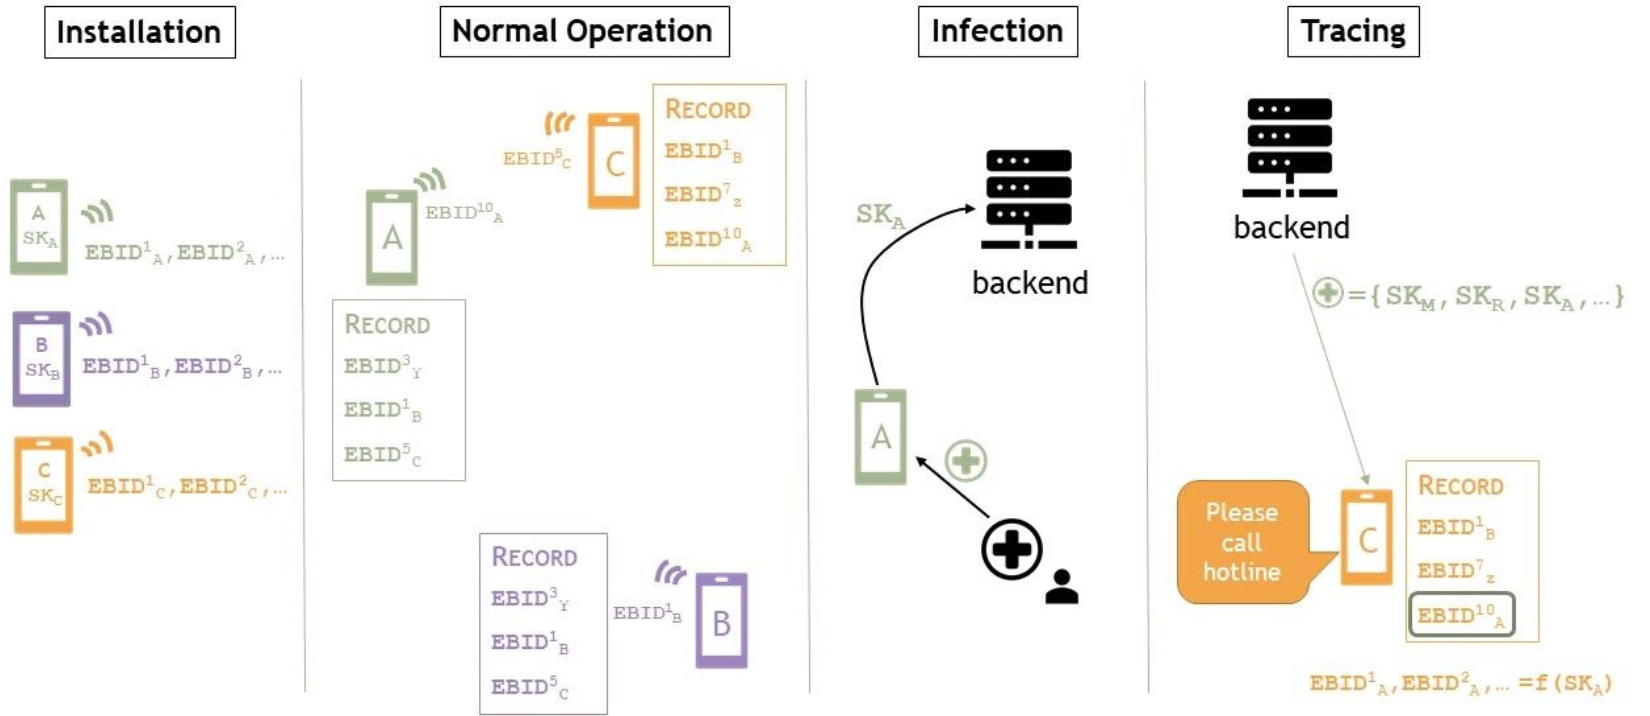
\includegraphics[scale=0.35]{fig/tracing_system}
\caption{Phases in the decentralized proximity tracing system}
\label{tracing_system}
\end{figure}
The system provides the following security and privacy protections:
\begin{itemize}\itemsep0pt
\item[-] \textbf{Ensures data minimisation}. (See below) No entity can observe or keep record of a global view of the social graph of a population, in anonymized form or otherwise.
\item[-] \textbf{Prevents function creep}. The entities in the system receive the minimum amount of information tailored to their requirements. None can abuse the data for other
purposes, nor can they be coerced or subpoenaed to make data available.
\item[-] \textbf{Protects non-infected users}. No entity, including the backend server, can learn information from non-infected users.
\item[-] \textbf{Graceful dismantling}. The system will organically dismantle itself after the end of the epidemic. Infected patients will stop uploading their data to the central server, and people will stop using the app. Data on the server is removed after 14 days.
\end{itemize}
And entails the following risks:
\begin{itemize}\itemsep0pt
\item[-] An \textit{active tech-savvy} adversary can reidentify EphIDs from infected people \textit{that they have been physically close to in the past} by actively modifying the app and collecting extra information about identities through additional means, such as a surveillance camera to record and identify the individuals. The information learned via the app is, in many cases, already expected to be known to this adversary (e.g., family, friends, neighbours, who will directly inform their close relations and friends). This attack \textbf{is inherent to any proximity-based system notification system}, as the adversary only uses the fact that they are notified together with additional information gathered by their phone or other means.
\item[-] A \textit{tech-savvy adversary} deploying an antenna to eavesdrop on bluetooth connections can learn which connections correspond to infected people, and then can estimate the percentage of infected people in a small radius of 50m. If in addition, the
adversary has a camera, he can capture images and potentially re-identify those people.
\end{itemize}
Both of these attacks are local: adversaries can learn (some) information about infected
individuals in close proximity to the equipment that they deployed.
\section*{High-Level Data Protection Overview}
Data protection by design and default obliges that:
\begin{quote}
\textit{only personal data which are necessary for each specific purpose of the
processing are processed. That obligation applies to the amount of personal
data collected, the extent of their processing, the period of their storage and
their accessibility (GDPR, art. 25)}
\end{quote}
There are five main data-protection-relevant actors in this system: \textbf{users , health
authorities , a backend server , epidemiological research projects , and mobile phone
operating system providers} (in this case, Apple and Google). Apple and Google only
provide a push notification service, the same as for any app and are aware that the app has been installed, acting as processors, but able to see no content or data. Nevertheless, since Apple and Google provide the operating system running on mobile devices, one has to trust them, since they could potentially learn information related to the proximity tracing system (who is infected, who infected whom, social graphs, etc.).


The decentralized approach notably minimises the amount of personal data collected by any
one entity, and heavily reduces the possibility of accessibility of any information, providing the guarantee that \textbf{the backend server learns nothing about identifiable individuals or their health status} . This promotes trust in the system, as concerns around function creep and lack of purpose-limitation (such as the repurposing of the protocol by law enforcement or intelligence services in countries in which it is deployed) can be solidly rebutted mathematically. This itself may lead to wider uptake.


The system is designed such that no entity beyond a user’s device processes or stores any
identifiable personal data about the user. As a whole, the system fulfils processing goals that would usually require personal data to be transmitted. \textbf{We believe that under normal operation, none of the data used to achieve proximity tracing need be characterised
as personal data, as no actors holding the data have the ability to re-identify it with
\textit{means reasonably likely to be used}} (following the test outlined by the CJEU in \textit{Breyer}).


The server transmits information about new infected ephemeral identifiers to users’ phones, which compute infection risk \textit{locally} , on the device. This comes with the important benefit that \textbf{the server cannot learn the social graph} , which is data that can easily be repurposed and misused in ways that individuals would not reasonably expect and may not wish. The proposed system guarantees that transmitted information cannot be used to identify an infected individual without a costly, illegal, and tightly geographically localised attack that \textit{was successfully carried out in the past, before the individual tested positive}. The theoretical potential of this attack is the tradeoff to obtain technical guarantees that prevent function creep and ensure limitation by design.


Because some theoretical attacks exist (above) — requiring high-effort, illegal activity to
carry out, and which only provide highly localised information — \textbf{we believe it is best for the purposes of trust to treat the entire pipeline with the same obligations that we would expect if personal data was processed by it}. There are additional ethical, non–data protection reasons to seek informed consent at every relevant point, although a
different lawful basis (e.g., task in the public interest) may be appropriate to rely on. As a result, the fact that the sensitive information, including health information, has equivalent protection to genuinely anonymous data, means that it is protected from all actors by among the most technically stringent safeguards possible in a system with the functions necessary for this purpose.
\clearpage
\section*{Detailed Stage-by-Stage Analysis}
\begin{quote}
\textit{In the remainder of the document, all communications between the app and the backend server, or any other party, are encrypted using the most appropriate TLS configuration.}
\end{quote}
\textbf{1. Installation process of proximity tracing app}


Users install the app from either the Apple App Store or the Google Play Store. No personal data is provided to the app.


\textit{Registering for push notifications}. The app needs to regularly receive information pertaining to newly infected patients from the backend server, so that it can locally determine whether its owner has been in physical proximity of an infected patient. Because apps running in the background are not guaranteed to be able to download information, the app registers for a push notification service: Firebase Cloud Messaging (FCM) on Android and Apple Push Notification service (APN) on iOS. The app sends the notification identifier to the backend. The backend stores this identifier to send information to the app. The backend does not store any other information (PII or otherwise) with this notification identifier.
\subsection*{Information security}
The mobile phone OS operators (Apple and Google) \textit{learn that the user installed the app} and have registered for the push notification service, but cannot see any data.


The backend server only stores the notification identifier of the app. This identifier is only used to \textit{send data} to the apps. When apps upload their seed SK after having been diagnosed, they do \textit{not}  supply this identifier to the backend.


Network observers only observe encrypted data between the app and the backend. This
data is the same for every app installation. Therefore network observers can conclude only
\textit{that somebody just installed the app}.
\subsection*{Data protection}
The main controller of the system (e.g. the coordinator of the backend server and app
deployment) would need a standard data processor agreement with the OS providers, as
with any public sector app using push notifications. The system envisaged here is unlikely to pose additional risks to the rights and freedoms of data subjects, as data subjects with smartphones will already be using these systems every day.


\textbf{2. Normal operation of proximity tracing app}


\textbf{Note: although we use the word ‘identifier’, the term used in data protection law, the technical specifications of the system prevent them from being used to identify
individuals}.


\textit{Broadcasting ephemeral Bluetooth identifiers}. Phones with the proximity tracing app installed broadcast ephemeral bluetooth identifiers (EphIDs) via Bluetooth low energy. These ephemeral identifiers are generated pseudo-randomly by the phone, derived from the secret key SK of the phone. EphIDs are rotated periodically. See Figure \ref{identifier}.


\textit{Storing of received Ephemeral Bluetooth Identifiers}. Phones receive Bluetooth identifiers that are being broadcasted by nearby phones. Phones store a record of each received ephemeral identifier with the following information:
\begin{itemize}\itemsep0pt
\item[-] Received EphID
\item[-] Coarse time window: morning/afternoon/night and the date
\end{itemize}
These records are stored locally on the phone and are \textbf{never} sent anywhere.


\textit{Pruning records}. Phones regularly delete records of old received EphIDs. They are stored no longer than the duration considered relevant by the health authority, anticipated to be 14 days, but this is reconfigurable.
\begin{figure}[H]
\centering
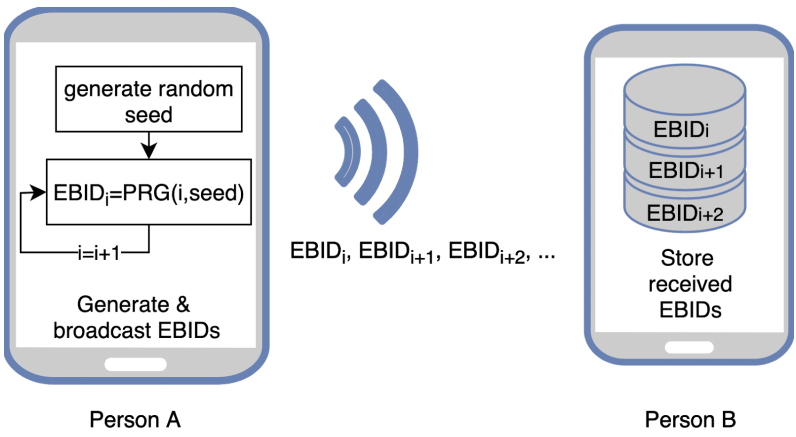
\includegraphics[scale=0.5]{fig/identifier}
\caption{Generation and broadcasting of ephemeral identifiers/EphIDs}
\label{identifier}
\end{figure}
\subsection*{Information security}
The EphIDs are generated pseudo-randomly and regularly rotated. Due to limitations on the
Bluetooth technology, EphIDs are sent in the clear. Yet, as they are random and rotated
frequently, they cannot be mapped to users’ identities nor be used to track them.


Apps of users that have not been diagnosed with SARS-CoV-2 can delete EphIDs after the
short period in which they are broadcasted, and will not further expose these EphIDs to the backend server. Only the confiscation of the phone, for example by law enforcement, might lead to the extraction of phone seeds to regenerate EphIDs of the given epoch. This risk can be mitigated by encrypting past seeds after they are used. These users are therefore not traceable based on EphIDs, even by parties that can receive and store these EphIDs. See below for the analysis for diagnosed patients.


Collected and broadcast EphIDs, and the underlying secret seeds, will not be exposed in the user interface of the app, as an additional safeguard against users seeking to go beyond normal operation.


From a traffic analysis perspective every instance of the app behaves the same. All of them broadcast ephemeral identifiers.
\subsection*{Data protection}
In normal operation, no user or the app on their phone processes personal data of any
individuals except themselves. While the information they collect, in conjunction with the broader protocol, enables them to compute a risk score, it does not relate to other identified or identifiable natural persons.


Users collect the ephemeral identifiers of nearby users who are using the app. These
identifiers are i) stored with only coarse time-frames (such as ‘the morning’), duration,
proximity, and other auxiliary data; and ii) rotating frequently. Future identifiers cannot be predicted from observing previous identifiers. Even if an individual takes note, records with a camera who they were near, and performs traffic analysis on the identifiers received during that time, they could not use that information to single out an individual at other times, or to re-identify data on others’ devices at other times. They would not learn more about non-infected individuals than they already knew: that they were present at a location at a specific time.


The only way to link a device across multiple broadcast identifiers is by using information held on that individual’s device. This would require access to that device, or obtaining recordings from the device. Doing so without permission would represent a computer misuse offence in most jurisdictions. The second scenario in which this information is provided is intentional and by design, during the calculation of whether an individual is at risk of infection. This situation is discussed further, below, when this aspect of the protocol is described. Neither situation will, however, reveal the identity of an individual unless there is side-information, e.g., a camera and on-device traffic analysis that stores the precise times that individuals met (not possible retroactively). This scenario is, however, not a flaw of the protocol, but rather a consequence of proximity tracking.


To underscore the data protective nature of these measures, it is worth noting that the
re-identification test set out by the CJEU in \textit{Breyer} (C-582/14) as necessary to classify this as personal data would not be met. Firstly, establishing an effective side-database would likely require breaking the law by surveilling individuals without an effective lawful basis (e.g. illegitimately using covert cameras directed outward from the person, see \textit{Ryneš} (C-212/13)). In \textit{Breyer} , the Court noted that the test of \textit{means reasonably likely to be used} to identify a natural person would not be met ‘if the identification of the data subject was prohibited by law’. Furthermore, it is also arguable that these specialised attacks would require ‘a disproportionate effort in terms of time, cost and man-power, so that the risk of identification appears in reality to be insignificant’ (\textit{Breyer}). However, as discussed, we suggest ensuring the obligations applying to personal data are still applied as good practice. Collecting emitted Bluetooth data would additionally trigger article 5(3) of the ePrivacy Directive, due to accessing/storing data from/on a terminal device. Multiple approaches to this are possible, but the simplest would be to obtain the informed consent of all users upon installation, which would then apply both ways, to the broadcast and the collection of EphIDs.


\textbf{3. Handling infected patients}


Health authorities diagnose patients that have been infected with SARS-CoV-2. After a
positive diagnosis, the health authority employee will ask the patient if they have the app installed, and if the patient is willing to reveal their EphID to facilitate contact tracing. If the user \textit{opts in},  they proceed as follows (see Figure \ref{infected}).
\begin{enumerate}\itemsep0pt
\item The health authority generates an authorization code for the patient, e.g., in the form of a QR code. The health authority shows this QR code to the patient.
\item The patient instructs her app to scan the QR code to obtain this authorization code.
\item The app opens an encrypted TLS connection to the server and sends the
authorization code and its seed SK, a compact representation of the EphIDs it has
broadcast during the infectious window, to the backend. The size of this message is
fixed. This upload does not  include the push-notification identifier.
\item When the backend receives the upload, it verifies the authorization code, and stores
the seed. It \textit{does not} store any other information related to the upload (such as IP addresses or time).
\end{enumerate}
\begin{figure}[H]
\centering
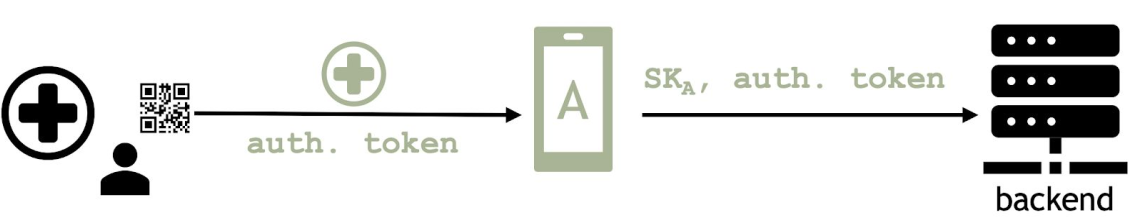
\includegraphics[scale=0.5]{fig/infected}
\caption{Information by infected patient}
\label{infected}
\end{figure}
To combat traffic analysis, apps periodically upload data to the server at predetermined
intervals (e.g., every 6 hours). If they are uploading the seed after being diagnosed, it
uploads the real EphID-representation and the authorization code. Otherwise, the app
transmits a dummy message formed by random bytes of the same size.
\subsection*{Information security}
Apps of users that have been diagnosed with SARS-CoV-2 send to the backend the seed of
their EphIDs corresponding to the infectious window. Given this seed, it is possible to link the EphIDs to the patient (whose identity is not revealed).\\[0.2cm]
Network observers can observe encrypted traffic between the phone and the backend.
However, the timing and schedule of this traffic is identical, regardless of whether the patient was infected or not.


\subsection*{Data protection}
\textbf{The health authority processes no additional personal data other than what it would usually process when carrying out a COVID-19 test}. This is in line with the principles of data protection by design, data minimisation, purpose limitation, and security. Their role is simply to facilitate processing by the user through validating the test and authorising the transfer of data to the server, without being a conduit to the data themselves. It may be that, following the case-law, this leaves them with controllership duties despite never seeing personal data (see \textit{Wirtschaftsakademie Schleswig-Holstein} (C-49/17); \textit{Jehovan todistajat} (C‑25/17); \textit{Fashion ID} (C-49/17)), however these would be minimal as they would already expect to be a controller in relation to the execution of the COVID-19 test. They shouldinform the user about the process, in line with GDPR art. 13, for example orally or with a sign.


\textbf{The backend server that the data is transmitted to cannot link any of the infected
EphIDs to natural persons}. In normal functioning, therefore, we can even understand that the server will not be holding personal data, although, as mentioned, we err on the side of caution and consider it to be personal data with near-anonymous safeguards. No additional data needs to be stored beyond these identifiers.


\textbf{4. Contact tracing and epidemiological research}


Several times a day, the backend server sends newly received EphID seeds of infected
patients to all installed proximity tracing apps via the notification service. This notification message also contains updates to the parameters of the local computation of the risk score of the device user, as well as information regarding calibration of the proximity computation.


Every device then proceeds as follows (see Figure \ref{risk}):
\begin{enumerate}\itemsep0pt
\item It compares the received EphIDs (corresponding to infected patients) to the stored
records of received Bluetooth identifiers.
\item If any of the received EphIDs matches a recorded identifier, the phone uses the latest parameters to compute a risk score based on the number of matching identifiers and
the total duration.
\item If the computed risk score is above the provided threshold, the app shows a
notification to the user that she/he has been in proximity to an infected patient. The
notification contains instructions on what to do and whom to contact.
\end{enumerate}
\begin{figure}
\centering
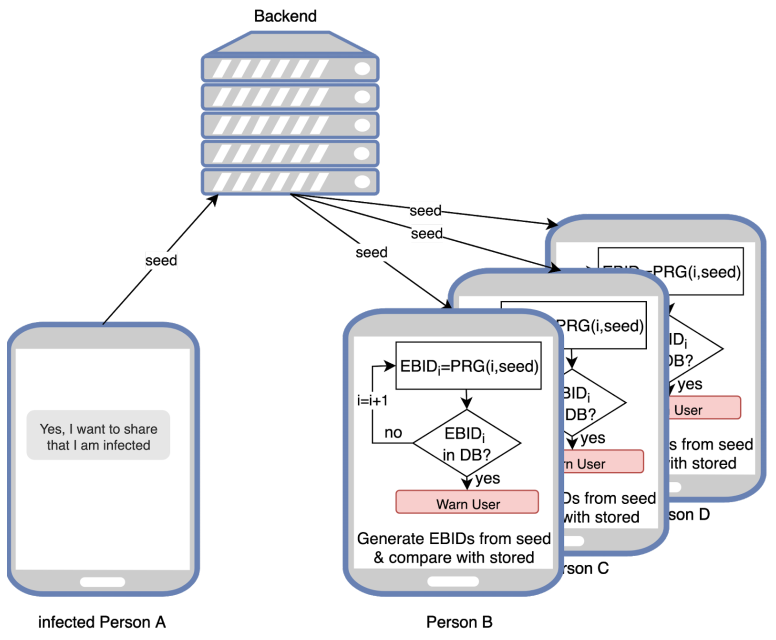
\includegraphics[scale=0.6]{fig/risk}
\caption{Warning of persons at risk}
\label{risk}
\end{figure}
\textit{Participating in epidemiology research} (Optional). During installation, the app asks the user if the user wants to participate in the epidemiology research to help understand the SARS-CoV-2 virus. If the user \textbf{opts in} , the app sends the following data to the epidemiology research lab at the next scheduled upload time:
\begin{itemize}\itemsep0pt
\item For each infected person (corresponding to an EphID seed, i.e. without revealing the
identity) that the smartphone observed: the number of encounters and the duration of
each contact.
\end{itemize}
To combat traffic analysis, apps will periodically upload data to the epidemiology research lab, even if they have not been in contact with an infected person. More precisely, the app picks a schedule for uploading data to the epidemiology research lab (e.g., once every 2 days). For every scheduled event, the phone creates an encrypted connection to the lab, and uploads either the real data, or a dummy message of the same size.
\subsection*{Information security}
The notification messages from the backend to the phones are encrypted. All phones
receive these messages. The phones process the received data locally, and if there is a
match they show a notification to the user without sending any information to any other
entity. Hence, from the perspective of an outside observer, the phones of both at-risk
persons, those who have been in contact with an infected person, and those who are not at
risk, behave the same.


Users who opt-in to the epidemiology research show a different traffic pattern. However, if a user has opted in to data sharing for research purposes, the app will regularly upload data to the epidemiology research lab so that an upload cannot be correlated with outside knowledge to detect whether a user has been in contact with an infected person.
\subsection*{Data protection}
The risk model that is transmitted is a simple formula that does not differ by individual, and therefore is not personal data. There are no data protection issues with its transmission.


As discussed above, from the server’s perspective, the data held is effectively not personal data, and cannot be linked back to individuals during normal operation. The user, upon downloading this non-personal data, computes a new category of personal data locally on their device: their risk score(s).


The data used to compute the risk score, by default, is held only on the device of the user. If the user opts in to sending this data for epidemiology research, the data they send contains few variables and no identifier among them, and would not be personal data when in the hands of the researchers.
\end{document}